\chapter{Model scenarios}
\label{chapter:model_scenarios}
introduction

\section{Model definition}
(representation of whcih nature)

This part of thesis is explorative. Not in correspondece with a single location. 
Hypotetical Northern Ghana situation outlined. Simplistic approach to succeed in the ability of upscaling . used to

aanname van cosntant head 2m verdegingen op basis van interview met locale bevolking 2 m lasting 4 months (entire wetseason) can be possible. 

aanname pomp op 30m, aanname etc  
 Deze scenarios kennen soms echter alsnog vaste aannames. De invloe hiervan zal worden bepaald middels sensitivity analysis. 

\subsection{Research time frame} 
4 months rainfall
8 months dry pumping

\subsection{Soil scenarios} 
explanation by image, ztop, zbot. unconfined, Sy, anistroy

\subsection{Well dimension \& daiy pump schedule}

\section{Modflow model construction}

\subsection{Modflow NWT} (mogelijk als intermezzo)

explanation about model dimension.. Appendix..
explanation about radial conversion.. Appendix
\textbf{layer and column precision}

\textbf{Scale of time}  

\textbf{Well definition}
size, depth, penetrations, 

\textbf{model built elements}
upw applied instead of lpf (gangbaar bij mf2005)
nwt instead of pcg (gangbaar bij mf2005)

\subsection{Modflow MNW2}

\textbf{parameter application} 
1 voor 1 uitleg omtrent de toegepaste parameters. 
Vertel hier ook over de gelimiteerde $Q_des$ middels $Q_thiem$.  

\subsection{Assumptions}

skin factor.. detailed explanation of use!

by the use of MNW2 there is more then multiple nodel connections invilved. This requires the introductuion of well resistance. NOne type not allowed. show equation and where the different components stand for. The A term no longer required. Is a scaling factor between well surface and cell service. Somethioing I did allraeady in my radial scaling. Moreover if the A factor would be applied. rw should be smaller than the representative ro value. This value is about 0.14m. System upscaling (3x initital diameter already exceeds this number. So model failure occurs. C term neglected in this case. Because of manual implementation of the CWC factor. Handy at the same time. Because the CWC of withdrawel can be equalled with the cond in the constant head infiltration period. 

B factor skin factor (reference USGS manual). Kskin typically smaller than kh. Since I'm only using this term to determine CWC it is even required to define Kskin smaller than Kh. If not the skin term and CWC term do become negative. Not allowed and model fails running. so Kskin should be scaled on the known Kh. It can be imagined the Kskin in conditions of low permable soil are relative more close to kh than when kh is better. For now assumption made for sc1 and 2 kskin slightly smaller than kh: kskin = 0.02 m/d. Same values applied for the other scenarios. This is highly arbitrairy. Future research should answer to what extent this assumption is correct. Although it is decisive on absolute ingoing and outgoing volumes. Still it is possible to make conclusions on trends due to upscaling. 

If xcan also take kskin values for the scenarios 3, 4 and 5 slightly smaller than the scenario kh values. But than highly unrealistic volumes are expected. Other option is to scale this bvy the use of the transmissivity values for example. kskin = kh * 1/ T for example. Own idea based on nothing. but than kskin values of respectively 0.022 and 0.021 will be used. Almost the same. \\

sc1b1: kskin groter dan kh kan niet. levert negatieve CWC en cond op. model fails
sc1b1: kskin = 0.02: failed to meet solver requirements
sc1b1: kskin = 0.01: Q-thiem (ongeveer 6.5 m3/d) wordt behaald als grens. hmin op -17.3 m (in de soil), hogere Q zou eventueel kunnen. Is een optie
sc1b1: kskin = 1/5 * kh: Q-thiem wordt op de eerste dag eventjes aangetikt. maar vervolgens elke dag niet meer. Mooi om deze te gebruiken denk ik zo.  voor sc1 (en 2 denk) facor van 1/5 toepassen. verhoog ik vervolgens de Q-des dan zie ik in de eerste tijdastapjes dus iets meer onttrekking. maar daarna  (vanaf dag2) alweer de zelfde Q waardes. Oftwel gelimiteerd door de hlim in de well. Mag ik dit zo doen. want Q-thiem is de Q die je moet onttrekken om op zeer lange termijn pompen een je hlim te bereiken. Nu begrens ik die zelf door hier mijn kskin op aan te passen waardoor ik die hlim (in well) nu al na enkele minuten bereik. Maar hoe anders te doen? \\

idee: die kskin aannemen die zorgt voor Q-thiem in eerste tijdstappen van eerste dag, maar in het vervolg worden losgelaten. Let op bij opschaling van diameter gaat je Q-thiem ook veranderen. \\


sc3b1: kskin = 1/5 * kh levert naar mijn mening al een vrij hoge conductance op. Q-thiem (nu ongeveer 171 m3/d, is dat niet wat hoog?). uitkomst toont aan: dat er ongeveer 20m3 per dag uitgehaald kan worden voor 243 dagen (et dat in 4 u pompen per dag. acht ik sterk onrealistisch. (alhoewel, dit is bij een volledig schoon systeem, wat niet het geval is in northern Ghana.. penlen vaak maar zo'n 10m). Desondanks verhoog ik de weerstand (verlaging conductance). daarom nu bij sc 3 voor kskin = 1/10 * kh gekozen. maar dan wordt Q-thiem iig nooit bereikt. \\


sc5b1: first try met kskin = 1/10 * kh. en Q-thiem is nu 652 m3/d, lijkt me wederom erg erg hoog. dus 1/25 * kh aangenomen. totaal niet wetenschappelijk verantwoord. Hoe dit op te lossen? \\


\section{Base model behaviour}

vertel welke base model is toegepast. Vertel vervolgens het process aan de hand van de meerdere head visualisaties en Q plots. (plot daarbij nog even de $Q_thiem$ lijn). 

doe voor 1 van de scenario's iets meer uitleg middels de plaatjes. (denk hier goed over  na, want wil wel plaatje zien met eerst een Q begrenzing en vervolgens (op het eind van dagelijks pompen niet meer!

laat vervolgens voor de 5 scenarios het base model uitkom zien middels een tabelletje met daarin voor de 5 scenarios dus. $Q_in_tot$, $Q_out_tot$ and $R\%$


\section{Upscaling}
waar het uiteindelijk om draait zijn de waardes van $Q_in_tot$, $Q_out_tot$ and $R\%$ tov het base model. So define new test criteria (opschaling tov het origineel/basemodel). iets van S(Q-in-tot)\% = (new/base)*(1/factor).. potentially intresting. Not strictly required. 


\tikzstyle{mybox} = [draw=black, fill=white, very thick,
    rectangle, rounded corners, inner sep=20pt, inner ysep=20pt]
\tikzstyle{title} =[fill=black, text=white]

\subsection{Upscaling by daily pumping time}

\begin{figure}[h]
\centering
\begin{tikzpicture}
\node [mybox] (box){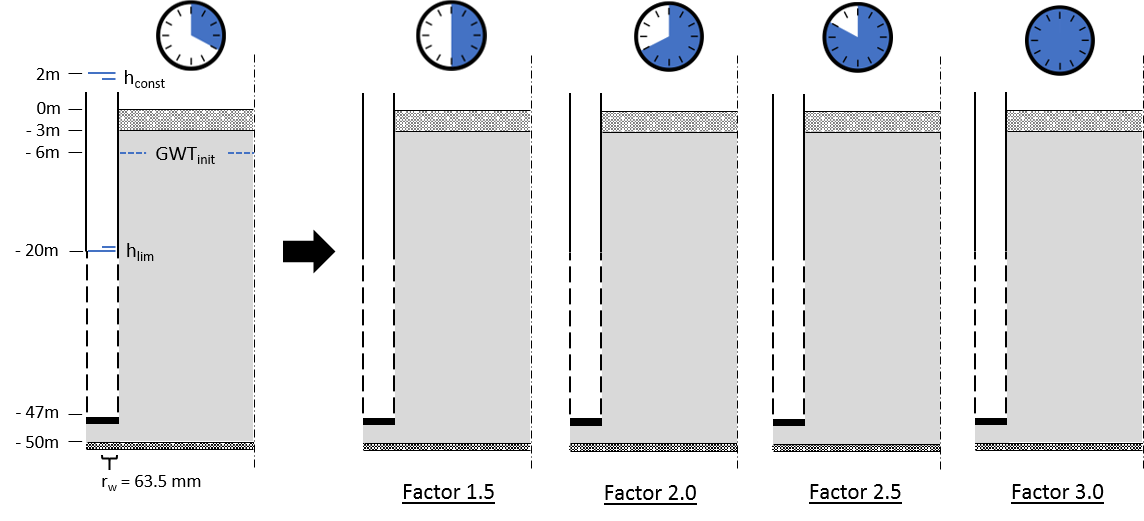
\includegraphics[width=0.9\linewidth]{Schematic_up_time}};  
\node[title, right=10pt] at (box.north west) {Schematic upscaling daily pumping time};
\end{tikzpicture}
\captionsetup{justification=centering}
\caption{Schematic upscaling daily pumping time}
\label{fig:Schematic_up_time}
\end{figure}

\begin{figure}[h!]
 \centering
 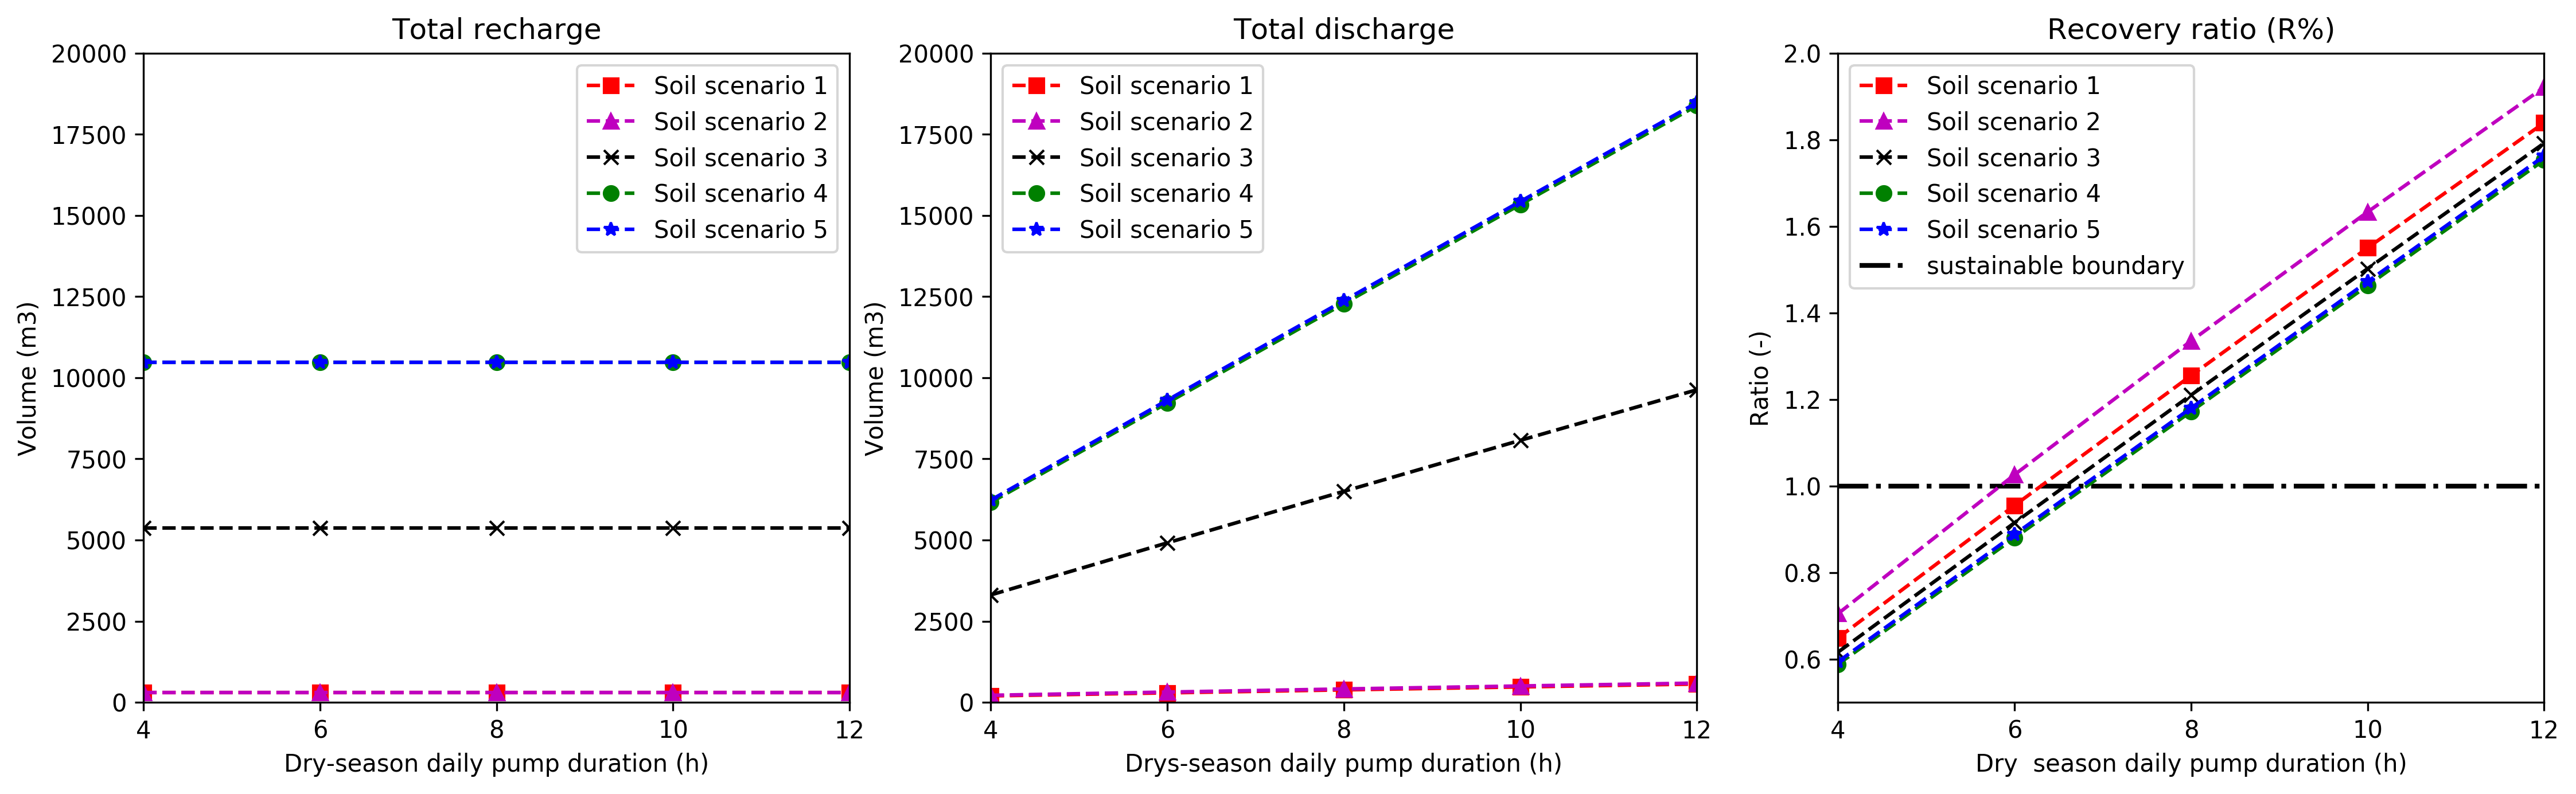
\includegraphics[width=1.0\linewidth]{Results_up_time}
 \captionsetup{justification=centering} 
 \caption{Results of yearly total volumes (in, out, ratio) by upscaling daily pumping time}
 \label{fig:Results_up_time}
\end{figure}

\subsection{Upscaling by borehole diameter}

\begin{figure}[h]
\centering
\begin{tikzpicture}
\node [mybox] (box){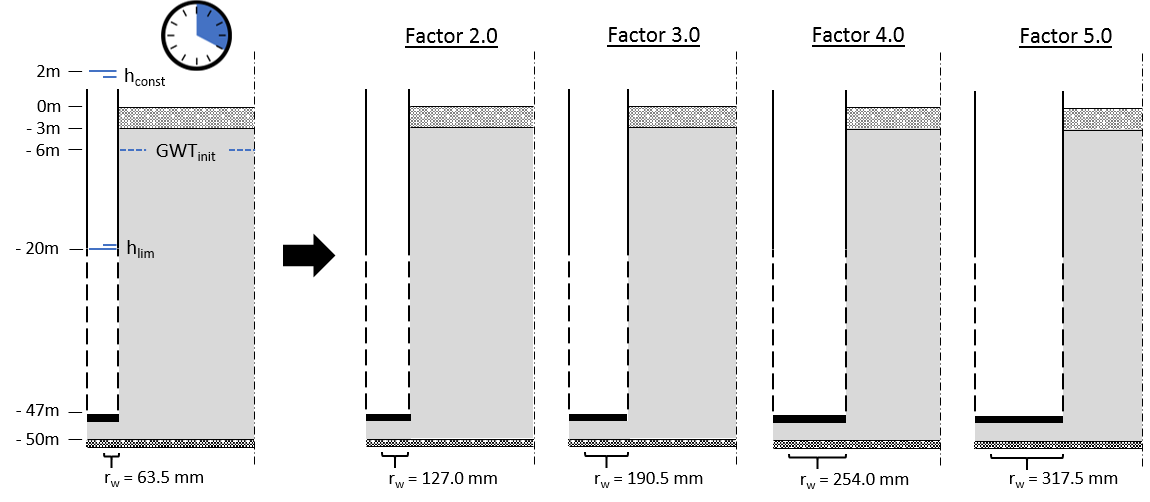
\includegraphics[width=0.9\linewidth]{Schematic_up_diam}};  
\node[title, right=10pt] at (box.north west) {Schematic upscaling well diameter};
\end{tikzpicture}
\captionsetup{justification=centering}
\caption{Schematic upscaling well diameter}
\label{fig:Schematic_up_diam}
\end{figure}

\begin{figure}[h!]
 \centering
 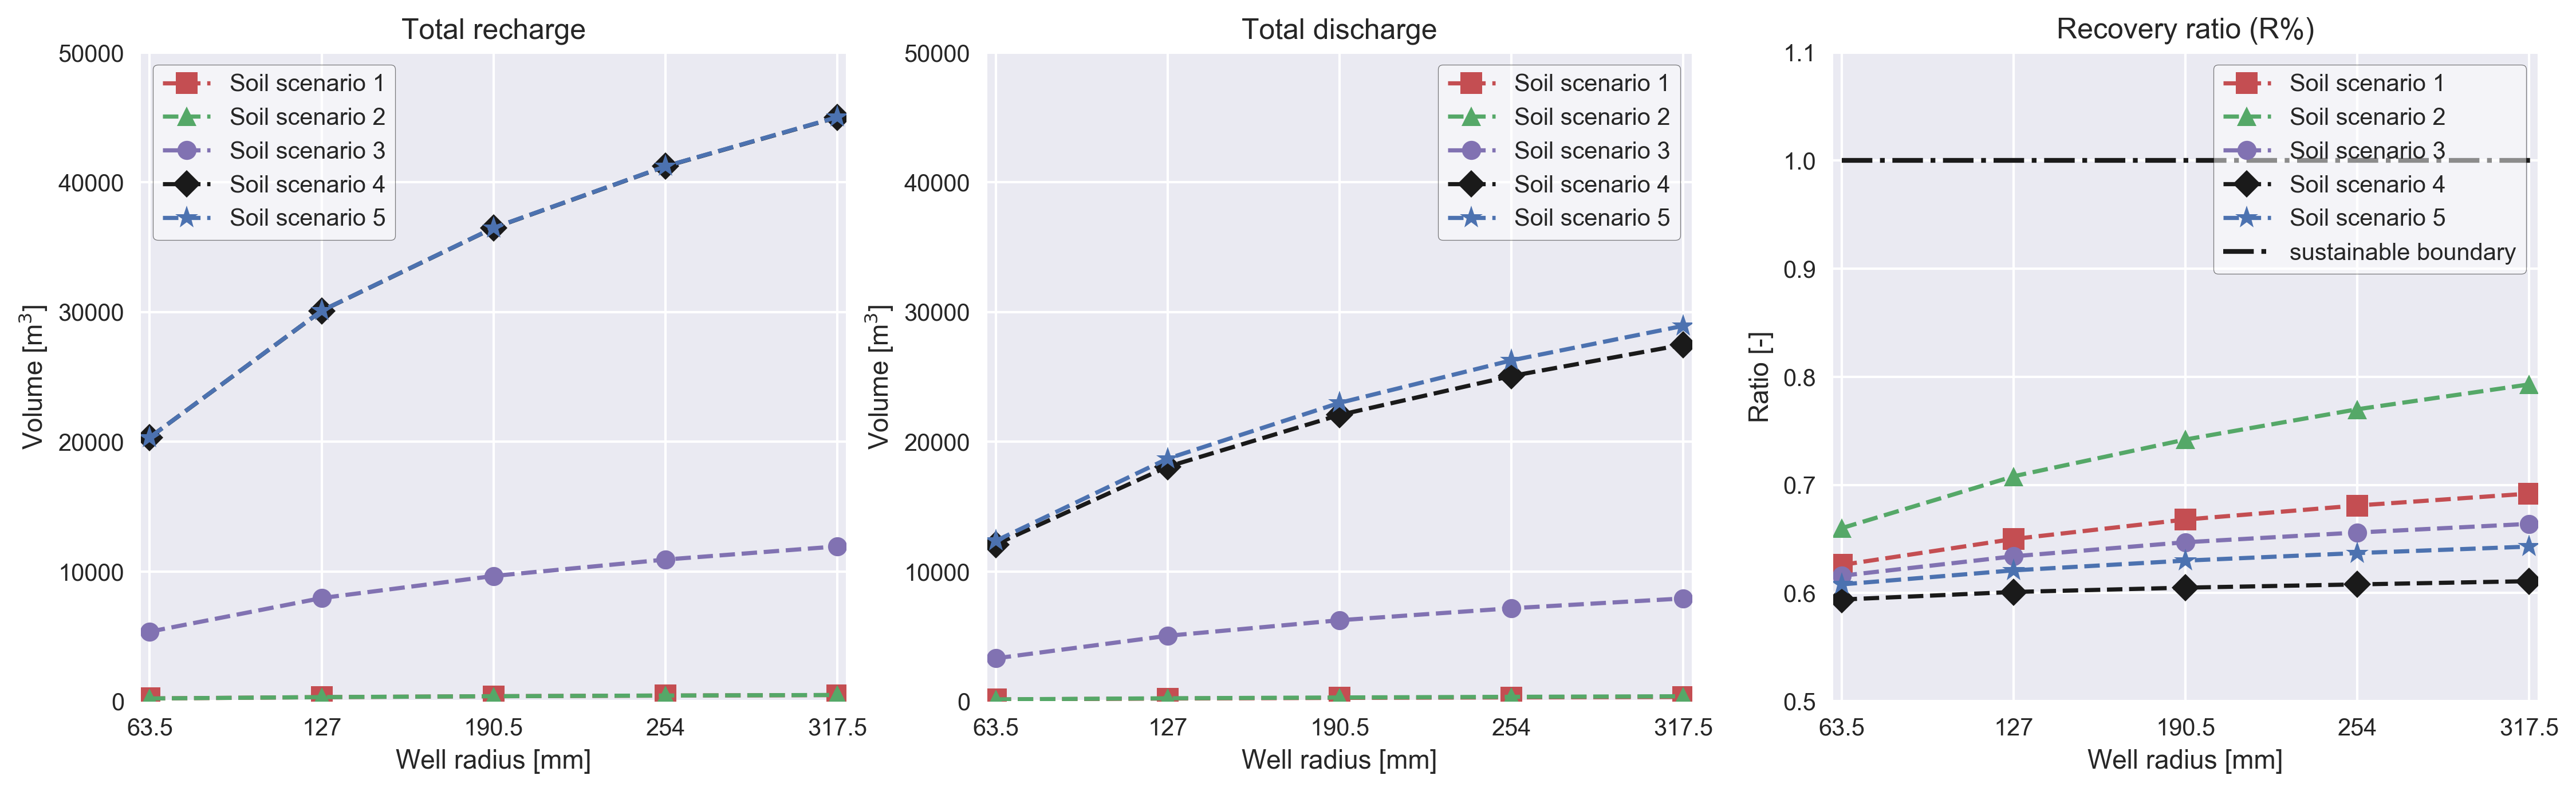
\includegraphics[width=1.0\linewidth]{Results_up_diam}
 \captionsetup{justification=centering} 
 \caption{Results of yearly total volumes (in, out, ratio) by upscaling well diameter}
 \label{fig:Results_up_diam}
\end{figure}


\subsection{Upscaling by cleaning}

\begin{figure}[h]
\centering
\begin{tikzpicture}
\node [mybox] (box){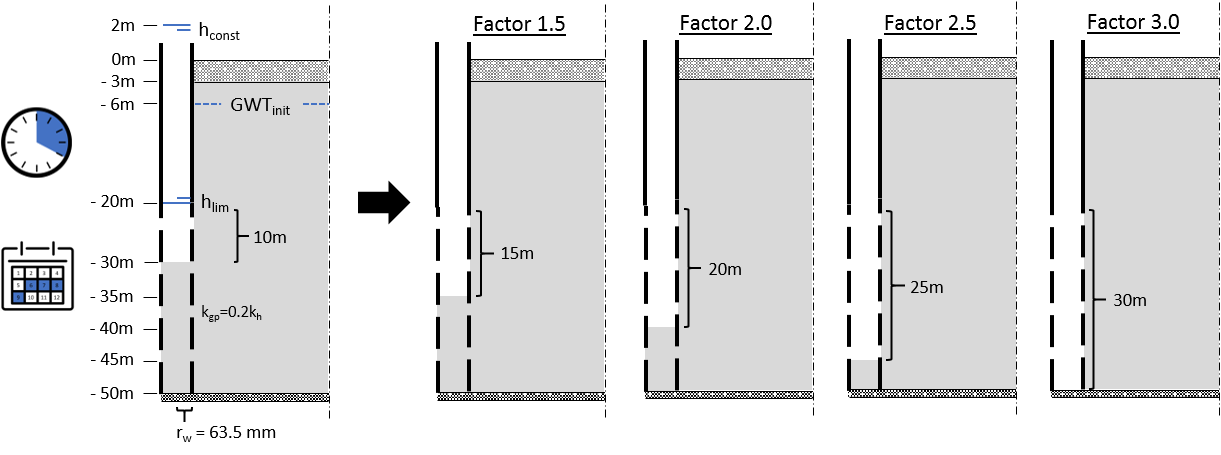
\includegraphics[width=0.9\linewidth]{Schematic_up_clean}};  
\node[title, right=10pt] at (box.north west) {Schematic upscaling well cleaning};
\end{tikzpicture}
\captionsetup{justification=centering}
\caption{Schematic upscaling penetration length due to well cleaning}
\label{fig:Schematic_up_clean}
\end{figure}


\begin{figure}[h!]
 \centering
 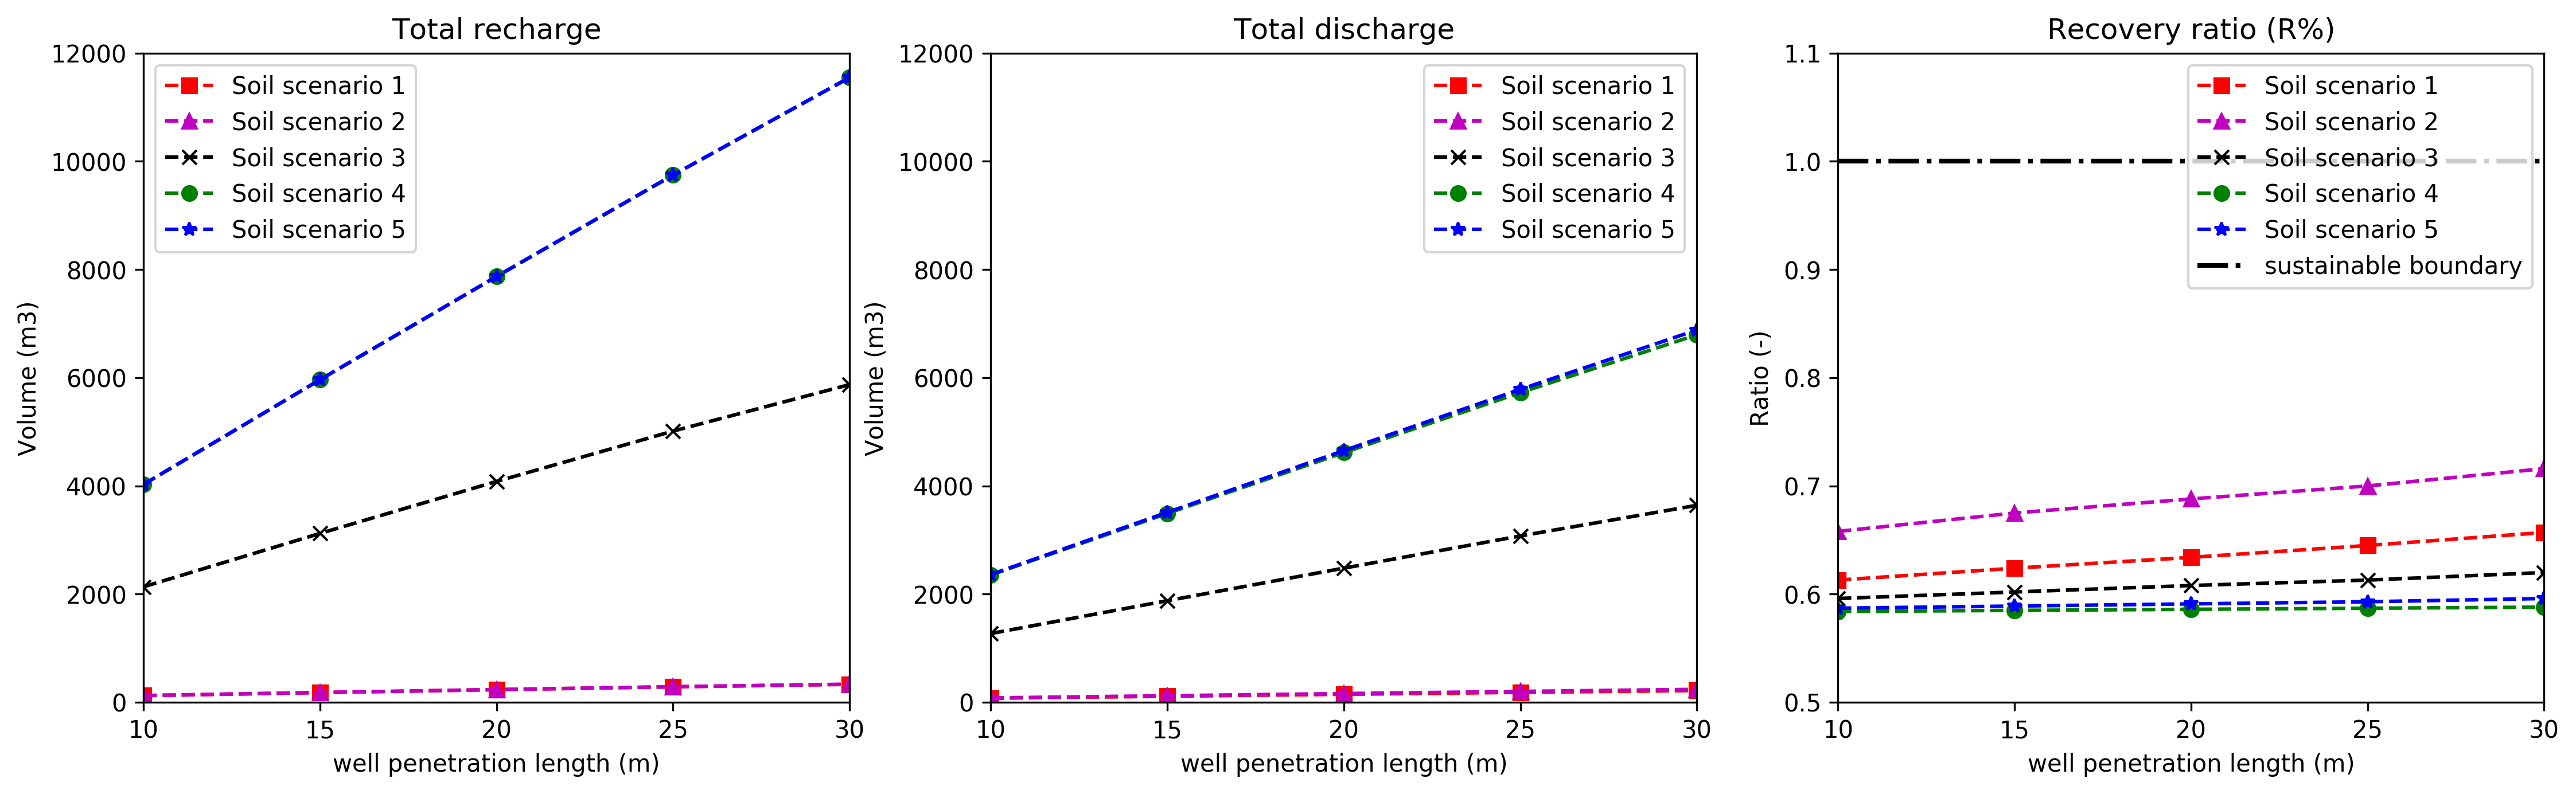
\includegraphics[width=1.0\linewidth]{Results_up_clean}
 \captionsetup{justification=centering} 
 \caption{Results of yearly total volumes (in, out, ratio) by upscaling the penetration length due to well cleaning}
 \label{fig:Results_up_clean}
\end{figure}


\section{Results \& Conclusions}
Korte samenvating dan wel conclusie over de vormen van opschaling. Wat het doet tov de basis. Misschien nog een schaling percentage doorvoeren 